\chapter{Termodinamica dei processi chimici}
Si pone ora l'attenzione sui fattori che governano il cambiamento chimico. La termodinamica si occupa di studiare sistemi macroscopici. La convenzione che verrà usata per tener conto delle variazioni di energia in un sistema chimico sarà la seguente.
\begin{notz}[convenzione segno variazione dell'energia di un sistema]\hfill
    \begin{itemize}
        \item Il calore fornito $Q$ o il lavoro $W$ fatto su un sistema è positivo.
        \item Il calore rimosso $Q$ o il lavoro $W$ fatto da un sistema è negativo.
    \end{itemize}
    Chiaramente, se un sistema guadagna una certa quantità di energia sotto forma di calore $Q$ dal suo intorno, la variazione sarà $+Q$ per il sistema e $-Q$ per l'ambiente. 
\end{notz}

\section{Energia interna}
Atomi e molecole che costituiscono la materia sono in continuo movimento e possiedono energia.
\begin{defn}[energia potenziale molecolare]
    La somma dell'energia cinetica e dell'energia potenziale definisce l'energia interna $U$.
\end{defn}
Scaldando un gas, le molecole si muovono più rapidamente, cioè hanno un maggior contenuto energetico. Se comprimiamo un gas, la sua pressione aumenta, il che implica nuovamente un maggior contenuto energetico. Queste considerazioni sono contenute in uno dei principi cardine della termodinamica.
\begin{axiom}[primo principio della termodinamica]
    Per un sistema isolato, la variazione di energia interna $U$, è la somma del calore $Q$ e del lavoro $W$, ovvero
    \begin{equation}\label{eq:I PdT}
        dU=dQ+dW.
    \end{equation}
\end{axiom}
Considerando il lavoro di espansione reversibile di un gas si può riscrivere l'equazione \eqref{eq:I PdT} come
\begin{equation}
    dU=dQ-pdV.
\end{equation}
Considerando un sistema a volume costante, la variazione di energia interna $U$ è
\begin{equation}
    \Delta U=Q+0=Q_V,
\end{equation}
dove il pedice $V$ indica che il processo avviene a volume costante. 

In altri termini la variazione di energia interna per un processo che avviene a volume costante in condizioni reversibili, corrisponde alla variazione di calore del sistema.
\begin{obs}
    Uno degli assunti di un gas perfetto è che le molecole siano
    sufficientemente distanti da non dare interazione. In questo modo l'energia interna dipende solo dalla temperatura e non dal volume del recipiente che contiene il gas o dalla sua pressione. Pertanto se si comprime il gas in modo isotermo, a $T$ costante, deve essere presente un trasferimento di calore dal sistema. Al contrario, un'espansione dev'essere accompagnata dall'assorbimento di calore dall'ambiente.
    \begin{equation}
        \Delta U=Q+W=0\quad\Rightarrow\quad Q=-W.
    \end{equation}
\end{obs}
\paragraph{Capacità termica dei gas.} Si può correlare la quantità di energia richiesta per scaldare una sostanza, considerando che, se una
quantità di energia $dQ_V$ addizionata ad un gas in condizioni di volume costante provoca un aumento di
temperatura $dT$.
\begin{defn}[capacità termica a volume costante]
    La capacità termica a volume costante $c_V$ è la quantità di calore necessaria per aumentare la temperatura di 1 mole di sostanza di 1 K a volume costante ed è data da
    \begin{equation}\label{eq:cap.term.V.cost}
        dQ_V=c_VdT\quad\therefore\quad c_V=\left(\frac{dQ}{dT}\right)_V.
    \end{equation}
\end{defn}
\paragraph{Misura della variazione di energia interna.} Come visto, se la reazione è condotta a volume costante, la variazione di energia interna è uguale alla variazione di calore. Ad esempio, la $\Delta U$ per una reazione di combustione può essere misurata con un calorimetro a volume costante, come quello in figura \ref{fig:Calorimetro a volume costante.}. La capacità termica del calorimetro $c_{cal}$ è data da
\begin{equation}
c_{cal}=\underbrace{m_{H_2O}}_{\substack{massa\\acqua}}c_{H_2O}+\underbrace{m_{steel}}_{\substack{ma  ssa\\acciaio}}c_{steel}.
\end{equation}
Se la combustione di $n$ moli di campione ha prodotto un incremento di temperatura $\Delta T$, la variazione $\Delta U$ è
\begin{equation}
    \Delta U_{comb}=-c_{cal}\frac{\Delta T}{n},
\end{equation}
dove il segno meno deriva dalla convenzione iniziale sui segni.
\begin{figure}[h]
    \centering
    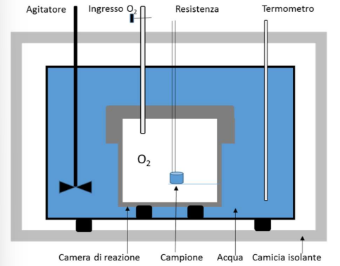
\includegraphics[width=0.5\linewidth]{Immagini/Calorimetro a volume costante.png}
    \caption{Calorimetro a volume costante}
    \label{fig:Calorimetro a volume costante.}
\end{figure}

\section{Entalpia}
La maggioranza delle reazioni chimiche viene condotta in condizioni di pressione costante. \'E quindi importante poter avere una funzione di stato che descriva le variazioni di energia in condizioni di pressione costante. Questa funzione è l'entalpia $H$. Si consideri una gas in un processo reversibile a pressione costante,
\begin{equation}
    \text{gas}(p,T_1,V_1),\,U_1\xleftrightarrow[p=costante]{}\text{gas}(p,T_2,V_2),\,U_2.
\end{equation}
L'energia può essere trasferita al sistema fornendo calore, o compiendo lavoro sul sistema. Quest'ultimo è dato, a pressione costante da $p\Delta V$. In queste condizioni, la variazione di energia a pressione costante è
\begin{equation}
    \begin{split}
        \Delta U=Q+W=Q_p-p\Delta V&\Rightarrow\Delta U+p\Delta V=Q_p \\
        &\Rightarrow\Delta U+\Delta(pV)=Q_p \\
        &\Rightarrow\Delta(U+p\Delta V)=Q_p \\
        &\Rightarrow\Delta H=Q_p,
    \end{split}
\end{equation}
da cui si deduce la seguente definizione.
\begin{defn}[entalpia]
    L'entalpia posseduta da un sistema termodinamico è una funzione di stato definita come 
    \begin{equation}
        H=U+pV.
    \end{equation}
\end{defn}
\begin{obs}
    La differenza tra $\Delta H$ e $\Delta U$
deriva dal termine $p\Delta V$. In generale la variazione di volume associata a liquidi e solidi è generalmente piccola e trascurabile. Per questi sistemi quindi $\Delta H\sim\Delta U$. Nel caso dei gas invece, le variazioni di volume possono essere molto rilevanti.
\end{obs}
Considerando le variazioni di entalpia, si usa la stessa convenzione dei segni adottata per l'energia interna.
\newpage
\begin{notz}[convenzione segno variazione dell'entalpia di un sistema]\hfill
    \begin{itemize}
        \item Processi che comportano uno sviluppo di calore sono detti esotermici e si ha $\Delta H>0$.
        \item Processi che comportano un assorbimento di calore sono detti endotermici e si ha $\Delta H<0$.
    \end{itemize}
\end{notz}
In analogia con l'equazione \eqref{eq:cap.term.V.cost} possiamo definire la capacità termica a pressione costante,
\begin{defn}[capacità termica a pressione costante]
     La capacità termica a pressione costante $c_p$ è la quantità di calore necessaria per aumentare la temperatura di 1 mole di sostanza di 1 K a pressione costante ed è data da
     \begin{equation}
         c_p=\left(\frac{dQ_p}{dT}\right)_p\quad\therefore\quad dH=c_PdT.
     \end{equation}
\end{defn}

\section{Variazioni di entalpia e legge di Hess}
L'entalpia è una funzione di stato. Una delle principali conseguenze è che la variazione di entalpia per una reazione chimica non è altro che la differenza tra lo
stato finale del sistema (i prodotti di reazione) e quello iniziale (i reagenti).
\begin{axiom}[Legge di Hess]
    La variazione totale di entalpia,per una reazione è indipendente dal cammino di reazione.
\end{axiom}
La legge di Hess (e il primo principio della termodinamica) ha importanti applicazioni in chimica. La conseguenza più ovvia è che $\Delta H_{diretta}=\Delta H_{inversa}$, ovvero, invertendo il senso di reazione,
cambia il segno di $\Delta H$. Un'altra conseguenza è la possibilità di calcolare variazioni di entalpia per
reazioni per le quali sarebbe difficile o impossibile ottenere un valore sperimentale.
\begin{ex}
    Consideriamo la reazione di ossidazio del monossido di carbonio CO a diossido di carbonio $\text{CO}_2$ alla pressione di 1 bar e a $\SI{25}{\celsius}$. 
    
    Si potrebbe fa avvenire la reazione direttamente in un calorimetro a $p$ costante e misura l'entalpia
    \begin{equation}
        {CO}_{\left(g\right)}+\frac{1}{2}{O_2}_{\left(g\right)}\to{CO_2}_{\left(g\right)},\quad\Delta H_1=-283.0\;\mathrm{kJmol^{-1}}.
    \end{equation}
    Alternativamente, è possibile valutare la reazione di ossidazione della grafite in presenza di ossigeno per le due reazioni.
    \begin{equation}
            \begin{cases}
            C_{(graf)}+\dfrac{1}{2}{CO_2}_{\left(g\right)}\to {CO_2}_{\left(g\right)},\quad\Delta H_2=-110.5\; \mathrm{kJmol^{-1}} \\
            C_{(graf)}+{O_2}_{\left(g\right)}\to {CO_2}_{\left(g\right)},\quad\Delta H_3=-393.5 \;\mathrm{kJmol^{-1}}
        \end{cases}.
    \end{equation}
    La legge di Hess, consente di trattare le equazioni chimiche su scritte come equazioni algebriche. Sottraendo la seconda dalla prima si ottiene
    \begin{equation}
    \begin{aligned}
            [C_{(graf)}+{O_2}_{\left(g\right)}]&-[C_{(graf)}+\frac{1}{2}{O_2}_{\left(g\right)}]\to[{CO_2}_{\left(g\right)}-{CO}_{\left(g\right)}]=\cdots\\
            &\cdots={CO}_{\left(g\right)}+\frac{1}{2}{O_2}_{\left(g\right)}\to{CO_2}_{\left(g\right)},
    \end{aligned}    
    \end{equation}
    con $\Delta H_3=\Delta H_1+\Delta H_2=-283.0\;\mathrm{kJmol^{-1}}$.
\end{ex}

\paragraph{Variazioni di entalpia.} La variazione di entalpia per una reazione chimica è semplicemente il calore assorbito o rilasciato quando la reazione avviene a pressione costante e corrisponde alla differenza di entalpia di prodotti e reagenti. Tuttavia, $\Delta H$ dipende dalla pressione e dalla temperatura a cui la reazione avviene, oltre allo stato dei componenti. \'E pertanto necessario definire un set di condizioni standard a cui fare riferimento. Questi sono: 
\begin{itemize}
    \item Pressione standard: 1 bar $=101325$ Pa.
    \item Temperatura standard: $25$ °C $=298.15$ K.
    \item Stato standard: componenti puri nello stato più stabile a 1 bar.
\end{itemize}
\begin{defn}[entalpia di reazione standard]
    L'entalpia di reazione standard è la variazione di entalpia in condizioni standard e la si indica con $\Delta H_{298}^{\circ}$.
\end{defn}

\paragraph{Entalpia di formazione standard.} La formazione di un composto a partire dai suoi elementi, come nell'esempio della reazione precedente, è
un'importante classe di reazioni.
\begin{defn}[entalpia di formazione standard]\label{defn:15}
        L'entalpia di formazione standard è la variazione di entalpia in condizioni standard per reazioni di formazione di un composto e la si indica con $\Delta H_f^\circ$.
\end{defn}
Poiché non è possibile definire un valore assoluto di entalpia, è necessario assumere un valore di riferimento. Per convenzione viene posto il valore di $\Delta H_f^\circ=0$ per gli elementi puri nei loro stati standard.
\begin{obs}
    In particolare, $\Delta H_f^\circ$ corrisponde alla variazione di entalpia quando 1 mole di un composto è formata in condizioni standard a partire dai suoi costituenti elementari nei loro stati standard.
\end{obs}
In generale, vale che
\begin{equation}
    \Delta H_{f,298}^\circ(reaz.)=\sum\nolimits_i\nu_{i}\Delta H_{f,298}^\circ(prod.)-\sum\nolimits_i\nu_i\Delta H_{f,298}^\circ(reag.),
\end{equation}
in cui $\nu_i$ rappresenta il coefficiente stechiometrico. Per la generica reazione $\alpha A+\beta B\to \gamma C+ \delta D$, si ha 
\begin{equation}
    \begin{aligned}
        \Delta H_{f,298}^\circ(reaz.)=[\gamma\Delta H_{f,298}^\circ(C)+\delta\Delta H_{f,298}^\circ(D)]-\cdots\\
        \cdots-[\alpha\Delta H_{f,298}^\circ(A)+\beta\Delta H_{f,298}^\circ(B)].
    \end{aligned}
\end{equation}
Possono essere definiti altri tipi di variazioni di entalpia:
\begin{itemize}
    \item Entalpia di combustione: definita semplicemente calore di combustione e corrisponde alla
    variazione di entalpia quando 1 mole di un composto reagisce completamente in presenza di un eccesso di ossigeno.
    \item Entalpie medie di legame:  rappresentano l'energia per mole necessaria per rompere un legame chimico in
    fase gas.
    \item Entalpie di transizione di fase.
\end{itemize}
\begin{obs}[entalpie di legame]
    E' importante realizzare che le entalpie di legame sono valori medi ottenuti da un gran numero di composti, vanno quindi considerati come approssimati.
\end{obs}

\section{Entropia}
La termodinamica non ci può dire nulla
relativamente alla velocità di un processo, ma tutto riguardo alla possibilità di avvenire di un processo e in che entità. Agli inizi della chimica fisica si pensava che la forza che guida un processo chimico ad avvenire fosse la
tendenza a minimizzare l'energia del sistema. Tuttavia le cose sono più complesse. Ad esempio, si consideri l'espansione di una gas ideale a temperatura costante. Non c'è variazione di energia, eppure il processo è spontaneo. La spontaneità di un processo è quindi determinato da un altro fattore oltre all'energia: l'entropia.
\begin{defn}[equazione di Boltzmann per l'entropia]
    L'entropia $S$ è definita da
    \begin{equation}
        S=k_B\ln{\omega},
    \end{equation}
    dove $\omega$ rappresenta il numero di possibili modi di organizzare il sistema e $k_B$ è la costante di Boltzmann.
\end{defn}
Da questa definizione si deduce che maggiore è il numero di stati accessibili, o meno ordinato è il sistema, maggiore è l'entropia. Ad ogni modo, la più grande utilità dell'entropia in chimica, è la possibilità di usarla per predire la direzione (spontaneità) di un processo chimico (o di qualunque altro processo).
    \begin{axiom}[secondo principio         della termodinamica]\label{ax:8}
        Un processo spontaneo comporta un incremento dell'entropia dell'universo.
    \end{axiom}
Dunque, Se determiniamo la variazione di entropia per un dato processo, saremo in grado di predirne la direzione e l'evoluzione.
\begin{obs}
     Considerando la relazione tra entropia e disordine, si può anche affermare che un processo spontaneo comporta un incremento del disordine.
\end{obs}
Quantitativamente, l'entropia può essere definita in base a considerazioni relativi a cicli lavoro-calore e sull'efficienza dei motori a combustione.
\begin{defn}[definizione quantitativa dell'entropia]
    La variazione di entropia $\Delta S$ è data da
    \begin{equation}\label{eq:entrop.quantitat.}
        \Delta S=\frac{Q_{rev}}{T},
    \end{equation}
    dove $Q_{rev}$ è una quantità di calore addizionata in modo reversibile alla temperatura $T$. 
\end{defn}
\begin{obs}
    La quantità $Q_{rev}$ è il massimo calore scambiabile, dunque l'entropia è associata alla massima variazione di energia a cui può essere soggetto un sistema.
\end{obs}
\'E possibile dimostrare che anche l'entropia è una funzione di stato: Pertanto, è lecito scrivere
\begin{equation}
    \Delta S=S_{finale}-S_{iniziale},
\end{equation}
indipendentemente dal percorso scelto.

La variazione di entropia durante un cambiamento di fase, fornisce una chiara applicazione dell'equazione \eqref{eq:entrop.quantitat.}, dal momento che, alla temperatura alla quale avviene la transizione di fase, il trasferimento di calore può essere considerato reversibile a pressione costante. Considerando la vaporizzazione e la fusione
possiamo scrivere
\begin{equation}\label{eq:sistema entrop.}
    \begin{cases}
        \Delta S_{vap}=\dfrac{\Delta H_{vap}}{T_{eb}}\\[2ex]
        \Delta S_{fus}=\dfrac{\Delta H_{fus}}{T_{fus}}.
    \end{cases}
\end{equation}
Chiaramente, $\Delta H_{vap}$ e $\Delta H_{fus}$ hanno segno positivo (reazioni endotermiche), pertanto $\Delta S$ sarà positivo per questi due cambiamenti di fase.

\paragraph{Entropia assoulta.} Le equazioni \eqref{eq:sistema entrop.}  permettono di calcolare la variazione di entropia per un qualunque composto che sia soggetto ad un cambiamento di fase, tuttavia non ci permettono di definire il valore di entropia in termini assoluti. \'E necessario quindi un valore di riferimento. Dalla definizione di entropia, uno standard a cui assegnare il valore zero può essere un cristallo solido perfetto a 0 K, anche se questa condizione è praticamente irraggiungibile.
\begin{defn}[terzo principio della termodinamica]
     L'entropia di un cristallo perfetto a $\SI{0}{\kelvin}$ è nulla.
\end{defn}

\paragraph{Variazioni di entropia.} Secondo le stesse modalità adottate per l'entalpia, possiamo definire l'entropia standard di reazione.
\begin{defn}[entropia standard di reazione]
    L'entropia standard di reazione $\Delta S_{298}^\circ$ è data da
    \begin{equation}
        \Delta S_{298}^\circ(reaz.)=\sum\nolimits_i\nu_i\Delta S_{298}^\circ(prod.)-\sum\nolimits_i\nu_i\Delta S_{298}^\circ(reag.).
    \end{equation}
\end{defn}
Per la generica reazione $\alpha A+\beta B\to\gamma C+\delta D$, si ha
\begin{multline}
\label{eq:entrp.reaz.std}
    \Delta S_{298}^\circ(reaz.)=[\gamma\Delta S_{298}^\circ(C)+\delta\Delta S_{298}^\circ(D)]- \\
    -[\alpha\Delta S_{298}^\circ(A)+\beta\Delta S_{298}^\circ(B)].
\end{multline}

\subsubsection{Entropia per predire la reattività chimica}
Si consideri la reazione
\begin{equation}
    2{\text{H}_2}_{\left(g\right)}+{\text{O}_2}_{\left(g\right)}\to2{\text{H}_2\text{O}}_{\left(l\right)}.
\end{equation}
Sostituendo i dati nell'equazione \eqref{eq:entrp.reaz.std} si ottiene
\begin{equation}
    \begin{split}
        \Delta S_{298}^\circ&=[2\times S_{298}^\circ({\text{H}_2\text{O}}_{\left(l\right)})]-[2\times S_{298}^\circ({\text{H}_2}_{\left(g\right)})+S_{298}^\circ({\text{O}_2}_{\left(g\right)})]=\cdots\\
        \cdots&=-327\;\text{kJmol}^{-1}.
    \end{split}   
\end{equation}
A seguito della reazione c'è quindi una forte diminuzione di entropia. Il risultato però non è consistente con l'esperienza e pare in netta contraddizione con il secondo principio della termodinamica.

L'apparente contraddizione nasce dal fatto che la seconda legge si riferisce all'entropia dell'universo, mentre nel calcolo su riportato ci siamo limitati a considerare il sistema. La variazione di entropia per la reazione, ovvero del sistema, è 571.6 kJmol$^{-1}$. Chiaramente, $\Delta H_{sist}^\circ=-\Delta H_{amb}^\circ$. Usando l'equazione \eqref{eq:entrop.quantitat.} si trova
\begin{equation}
    \Delta S_{amb}^\circ=\frac{\Delta H_{amb}^\circ}{T}=-\frac{\Delta H_{sist}^\circ}{T}=1920\;\text{JK}^{-1}mol^{1}.
\end{equation}
Considerando la variazione di entropia globale si ottiene
\begin{equation}
    \Delta S_{univ}^\circ=\Delta S_{amb}^\circ+\Delta S_{sist}^\circ=1593\;\text{JK}^{-1}mol^{-1}.
\end{equation}
Dunque, effettivamente l'entropia aumenta.

\section{Energia libera di Gibbs}
Le forze che guidano un processo chimico sono essenzialmente due: variazioni energetiche (entalpia e energia interna) e la tendenza di un sistema ad incrementare il disordine (variazione di entropia). Si vuole ora trovare la relazione tra questi due fattori. L'energia libera è una funzione che fornisce informazioni sulla spontaneità di un processo. L'idea dell'energia libera deriva direttamente dalla seconda legge della termodinamica. Per un processo spontaneo a pressione e temperatura costanti si ha
\begin{equation}
    \Delta S_{univ}=\Delta S_{amb}+\Delta S_{sist}>0.
\end{equation}
Questa relazione si riscrive come
\begin{equation}
    \Delta S_{univ}=\Delta S_{sist}+\frac{\Delta H_{amb}}{T}=\Delta S_{sist}-\frac{\Delta H_{sist}}{T}>0.
\end{equation}
Questa è un'equazione che si riferisce solo al sistema. Riarrangiando ed eliminando i pedici si ottiene
\begin{equation}
    \Delta H-T\Delta S<0.
\end{equation}
\begin{defn}[energia libera di Gibbs]
    La quantità $\Delta H-T\Delta S$ prende il nome di energia libera di Gibbs e si indica con $G$.
\end{defn}
\begin{obs}
    L'energia libera di Gibbs è la combinazione di due funzioni di stato, pertanto è anch'essa una funzione di stato.
\end{obs}
Quindi, la variazione di energia libera $\Delta G$ è 
\begin{equation}\label{eq:def.en.libera}
    \Delta G=G_{finale}-G_{iniziale}=\Delta H-T\Delta S.
\end{equation}
\'E chiaro quindi dall'equazione \eqref{eq:def.en.libera} che per un processo spontaneo a pressione e temperatura costante si deve avere
\begin{equation}
    {\left(\Delta G\right)}_{p,T}<0.
\end{equation}
\begin{obs}
    Un'analoga equazione può essere derivata considerando l'energia interna e cambiamenti energetici che avvengono a volume costante. In questo caso si definisce la funzione di Helmoltz (energia libera di Helmoltz) come
    \begin{equation}
        \Delta A=\Delta U-T\Delta S.
    \end{equation}
     Un cambiamento spontaneo in queste condizioni (temperatura e volume costanti) avverrà nel caso in cui $\Delta A<0$.
\end{obs}
\begin{axiom}[condizioni su $G$ per la spontaneità o meno di un processo]\hfill
    \begin{itemize}
        \item Se $\Delta G=0$, allora il sistema è all'equilibrio ed è reversibile.
        \item Se $\Delta G>0$, allora il processo non è spontaneo.
        \item Se $\Delta G<0$, allora il processo è spontaneo.
    \end{itemize}
\end{axiom}
\begin{figure}[h]
    \centering
    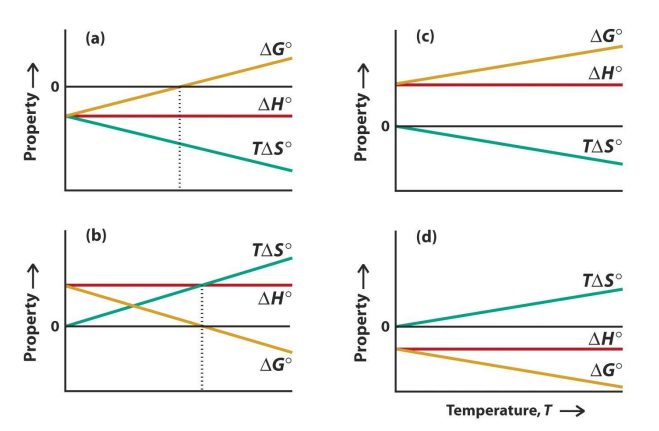
\includegraphics[width=0.65\linewidth]{Immagini/Contributi alla variazione dell'energia libera.png}
    \caption{casi di variazione di $G$ (c. mai spontanea, d. sempre spontanea).}
    \label{fig:enter-label}
\end{figure}
\paragraph{Energia libera di Gibbs di formazione.} Così come per l'entalpia di formazione standard (definizione \ref{defn:15}), possiamo definire l'energia libera di Gibbs di formazione standard.
\begin{defn}[energia libera di Gibbs di formazione standard]
    L'energia libera di Gibbs di formazione standard $\Delta G_{f}^\circ$ corrisponde alla variazione di energia libera di Gibbs quando 1 mole di un composto è formata a 298 K e 1 bar di pressione a partire dai suoi costituenti elementari nei loro stati standard.
\end{defn}
\begin{obs}
    L'energia libera di Gibbs di formazione standard fornisce anche un'importante informazione, relativa alla stabilità di un composto. Più $\Delta G_{f}^\circ$ è negativa, più stabile è il composto.
\end{obs}
\paragraph{Variazione di energia libera di Gibbs.} Un aspetto importante del problema, è la determinazione di come $\Delta G$ vari in funzione della variazione di temperatura e pressione e con la composizione del sistema. Si inizia considerando un sistema costituito da un unico componente. In questo caso si ha
\begin{equation}
    G=H-TS=(U+pV)-TS.
\end{equation}
Si consideri ora il differenziale totale $dG$ dato da
\begin{equation}
    dG=dU+pdV+Vdp-TdS-SdT.
\end{equation}
Ricordando che 
\begin{equation}
    \begin{cases}
        dU=dQ+dW=dQ-pdV \\
        dS=dQ/T\quad\therefore\quad dQ=TdS
    \end{cases},
\end{equation}
si ha
\begin{equation}\label{eq:diff.en.libera}
    dG=Vdp-SdT.
\end{equation}
Questa equazione ci permette di calcolare l'effetto sull'energia libera di Gibbs della variazione delle condizioni sperimentali. (pressione e temperatura).
\begin{caso}[variazione di $G$ in funzione di $T$ a $p$ costante]
        Consideriamo un processo condotto a pressione costante. Pertanto, $dP=0$ e si ha
        \begin{equation}\label{eq:var.G.pcost.}
            \left(\frac{\partial G}{\partial T}\right)_p=-S.
        \end{equation}
        In questo modo misurando la variazione di G in funzione della temperatura è possibile ricavare S. L'equazione \eqref{eq:var.G.pcost.} mostra che l'energia libera di Gibbs di un composto diminuisce all'aumentare della temperatura. Nel caso di una reazione chimica si deriva un'equazione analoga
        \begin{equation}
            \left(\frac{\partial\Delta G}{\partial T}\right)_p=-\Delta S.
        \end{equation}
\end{caso}
\begin{caso}[variazione di $G$ in funzione di $p$ a $T$ costante]
    Consideriamo un processo condotto a pressione costante. Pertanto, $dT=0$ e si ha
    \begin{equation}
        \left(\frac{\partial G}{\partial p}\right)_T=V.
    \end{equation}
    Nel caso di solidi e liquidi il volume di una mole varia poco in funzione di $p$ per cui $\Delta G$ è trascurabile. Invece, nel caso di un gas non è trascurabile. Considerando per semplicità un gas ideale si ha
    \begin{equation}
        \left(\frac{\partial G}{\partial p}\right)_T=V=\frac{nRT}{p}.
    \end{equation}
    Se $G$ varia da $G_1$ a $G_2$ per $p$ che varia da $p_1$ a $p_2$ si può scrivere
\begin{equation}\int_{G_1}^{G_2}dG=\int_{p_1}^{p_2}\frac{nRT}{p}=nRT\int_{p_1}^{p_2}\frac{dp}{p}\Rightarrow G_2-G_1=nRT\ln{\frac{p_2}{p_1}}.
    \end{equation}
    Infine, considerando la reazione in condizioni standard si ha
    \begin{equation}\label{eq:G(Gstd)}
        G=G^\circ+nRT\ln{\frac{p}{p^\circ}}=G^\circ+nRT\ln{a},
    \end{equation}
    dove $a$ è detta attività ed è un coefficiente adimensionale. Nel caso di solidi e liquidi, l'effetto della pressione è trascurabile e, per definizione $G=G^\circ$ per un liquido o solido puro, quindi per questi ultimi l'attività $a=1$.
\end{caso}
\begin{caso}[reazioni in soluzione]
    Nel caso di reazioni che avvengano in soluzione possiamo usare un'equazione analoga alla \eqref{eq:G(Gstd)} considerando la concentrazione del componente cui siamo interessati. Quindi,
    \begin{equation}
        G_i=G_i^{\circ}+nRT\ln{\bigg(\frac{[i]}{1\,\text{mol}}\text{dm}^{-3}}\bigg)=G_i^{\circ}+nRT\ln{[i]},
    \end{equation}
    dove $[i]$ indica la concentrazione dell'i-esimo componente.
\end{caso}

\subsection{Quoziente di reazione}
In realtà $\Delta G$ fornisce un
informazione molto più importante e dettagliata. L'energia libera cambierà durante la reazione a seconda delle proporzioni tra reagenti e prodotti ma raggiungerà un minimo per una qualche proporzione di prodotti e reagenti. A questo valore di minimo la reazione non avrà alcuna tendenza spontanea a procedere in nessuna direzione, raggiungendo l'equilibrio.
\begin{figure}[h]
    \centering
    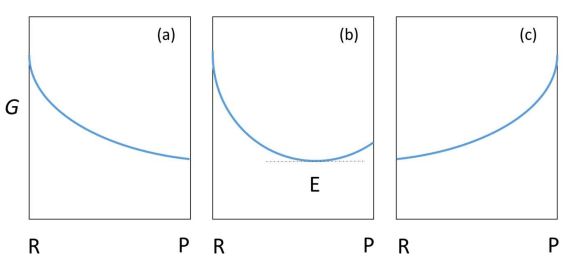
\includegraphics[width=0.6\linewidth]{Immagini/Variazione G durante reazione.png}
    \caption{variazione di $G$ durante una reazione (a. completa, b. equilibrio, c. non avviene).}
    \label{fig:Variazione G durante reazione}
\end{figure}

\begin{defn}[equilibrio chimico]
    Un sistema è all'equilibrio quando ha raggiunto un minimo nella sua energia libera.
\end{defn}
Chiaramente è importante avere una determinazione quantitativa della composizione di una miscela di reazione. Uno degli approcci è quello di ricorrere alla legge di azione di massa e definire un quoziente di reazione $Q$.
\begin{defn}[quoziente di reazione]
    Per la generica reazione $\alpha A+\beta B\to\gamma C+\delta D$, il quoziente di reazione $Q$ dato da
    \begin{equation}
        Q=\frac{\alpha_C^\gamma a_D^\delta}{a_A^\alpha a_B^\beta}.
    \end{equation}
\end{defn}
Per mettere in relazione le attività $a$ con dei parametri misurabili si considerano le attività dopo che la reazione raggiunge l'equilibrio. Quindi, si ha
\begin{equation}
    Q_{eq}=\frac{\alpha_{C,eq}^\gamma a_{D,eq}^\delta}{a_{A,eq}^\alpha a_{B,eq}^\beta}=K_{eq}.
\end{equation}
La quantità $K_{eq}$ prende il nome di costante di equilibrio ed è anch'essa adimensionale.
\begin{obs}
     A seconda del sistema possono essere definite diverse costanti di equilibrio. Se $K_{eq}$ è calcolata per un sistema in fase gas:
     \begin{itemize}
         \item facendo uso delle pressioni parziali viene indicata come $K_p$;
         \item facendo uso delle concentrazioni viene indicata come $K_c$.
     \end{itemize}
\end{obs}
\begin{axiom}[direzione reazione]\hfill
    \begin{itemize}
        \item Se $\Delta G<0$ oppure $Q<K_{eq}$, allora la reazione procede da sinistra verso destra.
        \item Se $\Delta G>0$ oppure $Q>K_{eq}$, allora la reazione procede da destra verso sinistra.
        \item Se $\Delta G=0$ oppure $Q=K_{eq}$, allora la reazione è all'equilibrio.
    \end{itemize}
\end{axiom}

\subsection{Relazione tra \texorpdfstring{$\bm{\Delta G}$}{G} e \texorpdfstring{$\bm{K_{eq}}$}{K}}
Si consideri una generica reazione, in cui, per semplicità, i coefficienti stechiometrici sono unitari
\begin{equation}
    A+B\to C+D.
\end{equation}
La variazione di energia libera per questa reazione è
\begin{equation}
    \Delta G(reaz.)=\Delta G(prod.)-\Delta G(reag.)=(G_C+G_D)-(G_A+G_B).
\end{equation}
Applicando l'equazione \eqref{eq:G(Gstd)} ai componenti A,B,C e D, si ha
\begin{multline}
    \Delta G(reaz.)=(G_C^\circ+G_D^\circ)-(G_A^\circ+G_B^\circ)+ \\
    +RT[(\ln{a_C}+\ln{a_D})-(\ln{a_A}+\ln{a_B})],
\end{multline}
ovvero
\begin{equation}
    \Delta G(reaz.)=\Delta G^\circ(reaz.)+RT\ln{Q}.
\end{equation}
Quando la reazione raggiunge l'equilibrio si ha che $\Delta G(reaz.)=0$ e $Q=K_{eq}$. Pertanto,
\begin{equation}
    K_{eq}=e^{-\frac{\Delta G^\circ}{RT}}.
\end{equation}
\begin{obs}
    Lo stesso metodo, applicato a qualunque reazione con qualunque stechiometria porta allo stesso risultato.
\end{obs}
Idealmente, si definisce una reazione completata se fornisce il 99.99\% dei prodotti, ovvero se
\begin{equation}\label{eq:reaz.compl.}
    K_{eq}=\frac{quantit\grave{a}\,di\,prodotti}{quantit\grave{a}\,di\, reagenti}=\frac{99.99}{0.01}\approx10^4.
\end{equation}
Tuttavia, questa condizione è molto lontana dalla realtà. Per riassumere, usando entalpie e entropie standard, calcolando la variazione di energia libera e la costante di equilibrio, è possibile prevedere il decorso di una reazione, la posizione dell'equilibrio, e calcolare la massima quantità di prodotti ottenibili.

\section{Potenziale chimico}
\label{sec: potenziale chimico}
Ora ci si concentra sul come varia l'energia libera quando un componente è addizionato ad un sistema in cui tutte le altre condizioni e quantità di componenti sono mantenute costanti. Matematicamente questo è espresso dal differenziale parziale di $G$ rispetto a quel componente.
\begin{defn}[potenziale chimico]
    Il nome di potenziale chimico $\mu_A$ di un componente A è dato da
    \begin{equation}
    \mu_A=\left(\frac{\partial G}{\partial n_A}\right)_{p,T,n_B},
\end{equation}
dove $\mu_A$ rappresenta la variazione di energia libera quando una mole di A è addizionata ad un sistema in cui le altre condizioni sono mantenute costanti.
\end{defn}
Se si aggiunge un piccola quantità $dn_A$ ad una sostanza B, la variazione di energia libera a temperatura e pressione costante è
\begin{equation}
    dG=\mu_Adn_A.
\end{equation}
L'equazione \eqref{eq:diff.en.libera} può essere ulteriormente generalizzata includendo la variazione di composizione che caratterizza una reazione chimica
\begin{equation}
    dG=Vdp-SdT+\sum\nolimits_i\mu_idn_i.
\end{equation}
Si consideri ora una reazione del tipo $A\to B$. Se la reazione consiste in $dn$ moli di A che reagiscono formando $dn$ moli di B, allora $dG$ è data da
\begin{equation}
    dG=-\mu_Adn+dn=dn\left[-\mu_A^\circ-RT\ln{\frac{p_A}{p_A^\circ}}+\mu_B^\circ+RT\ln{\frac{p_B}{p_B^\circ}}\right].
\end{equation}
Ricordando che $p_A^\circ=p_B^\circ=1$ bar, si ha
\begin{equation}\label{eq:dG/dn}
    \frac{dG}{dn}=\mu_B^\circ-\mu_A^\circ+RT\ln{\frac{p_B}{p_A}}.
\end{equation}
All'equilibrio $dG/dn=0$ e $p_B/p_A=k_{eq}$, da cui si deriva l'equazione \eqref{eq:reaz.compl.}. Inoltre, dall'equazione \eqref{eq:dG/dn} si trova che quando la reazione raggiunge l'equilibrio $\mu_A=\mu_B$.
\begin{defn}[equilibrio a temperatura e pressione costante]
    Una reazione raggiunge l'equilibrio a temperatura e pressione costante, quando il potenziale chimico dei reagenti eguaglia quello dei prodotti.
\end{defn}
Per riassumere,  il potenziale chimico può essere visto come la forza che guida un processo chimico.

\subsection{Relazione tra \texorpdfstring{$\bm{K_{eq}}$}{K} ed esperimento}
\'E possibile mettere in relazione la costante di equilibrio con con la quantità di reagenti e prodotti che partecipano alla reazione.
Consideriamo ad esempio la reazione 
\begin{equation}
    {\text{N}_2\text{O}}_{\left(g\right)}\longleftrightarrow{2\text{N}_2\text{O}_4}_{\left(g\right)}.
\end{equation}
Se una mole dei reagenti è è introdotta in un contenitore e il sistema lasciato andare all'equilibrio ad una pressione
totale di equilibrio $p_{TOT}$, possiamo dire che $\alpha$ moli hanno reagito. Quindi, il numero totale di moli di gas presenti sarà dunque $(1-\alpha)+2\alpha=2\alpha$. Dalla definizione di $K_{eq}$ si ha
\begin{equation}
    K_p=\frac{\left({{p_{(prod.)}}/{p_{(reag)}^\circ}}\right)^2}{{p_{(reag.)}}/{p_{(prod.)}^\circ}}.
\end{equation}
Facendo uso delle frazioni molari definite come
\begin{equation}
    \chi=\frac{moli\,del\,componente}{moli\,totali},
\end{equation}
si trova
\begin{equation}
    K_p=\frac{\left(\chi_{(prod.)}p_{TOT}\right)^2}{\chi_{(reag.)}p_{TOT}}=\left(\frac{2\alpha}{1+\alpha}\right)^2\left(\frac{1-\alpha}{1+\alpha}\right)p_{TOT},
\end{equation}
da cui
\begin{equation}
    K_p=\frac{4\alpha^2p_{TOT}}{1-\alpha^2}.
\end{equation}
Anche se il metodo è molto potente, l'espressione di $K_p$ dipende dalla stechiometria con cui la reazione è scritta e le equazioni risultanti possono essere difficili da risolvere per via analitica. Assumendo che il grado di avanzamento
della reazione sia piccolo, $\alpha\ll1$ e $1-\alpha\approx1$, quindi 
\begin{equation}
    K_p\approx4\alpha^2p_{TOT},\qquad\alpha\approx\sqrt{\frac{K_p}{4p_{TOT}}}.
\end{equation}

\subsection{Effetto delle condizioni esterne su \texorpdfstring{$\bm{K_{eq}}$}{K}}
Uno degli obiettivi principali quando si progetta una reazione chimica è quello di massimizzare la resa di
reazione.
\paragraph{Effetto della pressione.} Un fraintendimento frequente è quello che la costante di equilibrio dipenda dalla pressione del sistema. Non
è così. $K_{eq}$ dipende da $\Delta G^\circ$ che è valido solo a 1 bar. Pertanto, $K_{eq}$ è una costante termodinamica
che non varia a temperatura costante. Questo però non vuol dire che la pressione non abbia un effetto sulla
posizione dell'equilibrio. Consideriamo la reazione del precedente paragrafo e la relativa
\begin{equation}
    K_p\approx4\alpha^2p_{TOT}.
\end{equation}
Se $K_p$ dev'essere costante, nel caso in cui $p_{TOT}$ cambi, anche $\alpha$ deve cambiare in modo da compensare. Dall'espressione di $K_p$ si vede che se la pressione totale aumenta, il grado di dissociazione di $\text{N}_2\text{O}_4$  deve diminuire, per compensare. In questo modo anche
la resa del prodotto diminuisce.
\paragraph{Effetto della temperatura.} Ricordando che
\begin{equation}
    \begin{cases}
        \Delta G=\Delta H-T\Delta S \\
        \Delta G=\Delta G^\circ+RT\ln{Q} \\
        \Delta G+RT\ln{K_{eq}}=0,\; \mathrm{all'equilibrio}
    \end{cases},
\end{equation}
si ricava che
\begin{equation}
    \ln{K_{eq}}=\frac{\Delta S^\circ}{R}-\frac{\Delta H^\circ}{RT}.
\end{equation}
Questa equazione è una variante dell'equazione di Van't Hoff. Assumendo che $\Delta H^\circ$ e $\Delta S^\circ$ non varino in maniera significativa nell'intervallo di temperatura studiato si ottiene una relazione lineare tra $K_{eq}$ e $1/T$. Alternativamente, conoscendo i valori di $K_{eq}$ a due temperature si può scrivere
\begin{equation}
    \ln{\frac{K_{eq}\left(T_2\right)}{K_{eq}\left(T_1\right)}}=\frac{\Delta H^\circ}{R}\left(\frac{1}{T_1}-\frac{1}{T_2}\right).
\end{equation}
Da questa relazione si vede che per una reazione esotermica ($\Delta H<0$) la costante di equilibrio $K_{eq}$ diminuisce
all'aumentare di $T$ ovvero la reazione si sposta verso la formazione dei reagenti. L'opposto è vero per una reazione endotermica.

L'effetto di una variazione nelle condizioni esterne, sull'equilibrio di una reazione chimica, è sinteticamente
espresso nel seguente principio
\begin{axiom}[principio di Le Chatellier]
    Se si alterano le condizioni esterne di un sistema termodinamico, l'equilibrio del sistema tende a
spostarsi in modo da opporsi al cambiamento delle condizioni esterne. 
\end{axiom}
Per riassumere, considerando una reazione esotermica, se la temperatura aumenta, il sistema evolverà in modo da assorbire l'energia fornita, minimizzando la quantità di energia prodotta dalla reazione. La reazione quindi si sposta verso la formazione di reagenti e la resa dei prodotti diminuisce. Ovviamente è vero l'opposto nel caso di una reazione endotermica, in cui la formazione di prodotti sarà incrementata dall'aumento di temperatura.

\section{Termodinamica della cella elettrochimica}
Le reazioni di ossido – riduzione, costituiscono un'importante classe di reazioni, che possono essere sfruttate per compiere lavoro elettrico (pile). Ad esempio se un pezzo di zinco è immerso in una soluzione contenente ioni rame (ad esempio una soluzione di solfato di rame) lo zinco si ricopre rapidamente di un deposito bruno di rame metallico. La reazione chimica che avviene è
\begin{equation}
    \textnormal{Zn}_{\left(s\right)}+\textnormal{Cu}_{\left(aq\right)}^{2+}\to\textnormal{Cu}_{\left(s\right)}+\textnormal{Zn}_{\left(aq\right)}^{2+}.
\end{equation}
Se le reazioni di ossidazione e riduzione sono fatte avvenire in due comparti separati (anche se connessi per permettere il trasporto di carica) gli elettroni possono essere fatti fluire in un circuito esterno.
\begin{figure}[h]
    \centering
    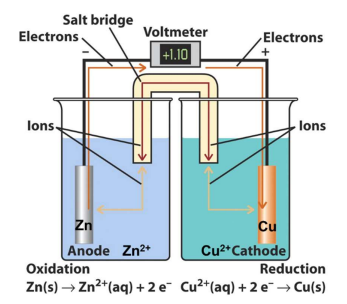
\includegraphics[width=0.5\linewidth]{Immagini/Pila Daniell.png}
    \caption{pila Daniell.}
    \label{fig:Pila}
\end{figure}
\subsubsection{Potenziali elettrochimici standard}
La differenza di potenziale generata, dipende dalla natura delle due semicelle. Il potenziale zero è assegnato ad una semicella in cui avviene la reazione di riduzione dell'idrogeno
\begin{equation}
    \textnormal{H}_{\left(aq\right)}^+ +e\to\frac{1}{2}{\textnormal{H}_2}_{\left(g\right)},
\end{equation}
in condizioni standard. I potenziali di elettrodo misurati in queste condizioni sono indicati con il simbolo $E^\circ$, mentre $E$  indica la differenza di potenziale quando la cella opera in condizioni diverse da quelle standard. Questa differenza di potenziale è una misura della tendenza che gli elettroni hanno a fluire nel circuito, il che corrisponde alla tendenza che la reazione ha ad avvenire spontaneamente. Questa tendenza è legata a $\Delta G$, quindi deve esistere una relazione tra $E$ e $G$.

Si considerino $n$ elettroni che vengono trasferiti in una reazione redox. La carica totale $Q$ sarà data da $nF$, dove $F$ è la costante di Faraday uguale a 96485 C mol$^{-1}$. Una carica $Q$ che si muove attraverso una differenza di
potenziale $E$, compie un lavoro dato da
\begin{equation}
    W_{el}=-\int_{Q_i}^{Q_f}EdQ.
\end{equation}
Se la differenza di potenziale – voltaggio – è costante, il lavoro associato al trasferimento di carica è
\begin{equation}
    W_{el}=-nFE.
\end{equation}
In condizioni di temperatura e pressione costante, questo lavoro è il risultato della diminuzione dell'energia libera di Gibbs mentre il sistema raggiunge l'equilibrio. Pertanto si può scrivere
\begin{equation}\label{eq:G(E)}
    \Delta G=-nFE.
\end{equation}
Nel caso in cui tutti i componenti siano nei loro stati standard avremo
\begin{equation}\label{eq:G(Estd)}
    \Delta G^\circ=-nFE^\circ.
\end{equation}
Dato che $E$ e $G$ hanno segno opposto, una reazione è spontanea se $E>0$.

\subsubsection{Dipendenza dei potenziali di elettrodo dalla concentrazione}
Si è visto che la variazione di energia libera di Gibbs è data da
\begin{equation}
    \Delta G=\Delta G^\circ+RT\ln{Q}.
\end{equation}
Sostituendo le equazioni \eqref{eq:G(E)} e \eqref{eq:G(Estd)} si ottiene
\begin{equation}
    -nFE=-nFE^\circ+RT\ln{Q},
\end{equation}
da cui
\begin{equation}
    E=E^\circ-\frac{RT}{nF}\ln{Q}.
\end{equation}
Questa equazione prende il nome di equazione di Nernst. Quando la cella è in equilibrio $\Delta G=E=0$, quindi 
\begin{equation}
    E^\circ= \frac{RT}{nF}\ln{K_{eq}}.
\end{equation}
Questa è un'equazione è molto utile per calcolare $K_{eq}$ dato che sono noti molti valori di $E^\circ$ per un enorme numero di reazioni.

\section{Equilibri di fase}
Per prima cosa è necessario dare una definizione precisa di fase.
\begin{defn}[fase di un sistema]
    Una fase è una parte omogenea di un sistema, con composizione chimica determinata e proprietà fisiche uniformi, separata da altre parti del sistema da superfici limite fisicamente definite. 
\end{defn}
Nel caso di gas e vapori può esistere una sola fase, indipendentemente dal numero di componenti del sistema. Per un componente singolo ci può essere solo una fase liquida, mentre nel caso di un solido queste possono essere più di una.

Come già visto, un sistema tenderà sempre ad evolvere verso uno stato in cui è minima l'energia di Gibbs. Per un componente singolo, puro, la dipendenza dell'energia libera di Gibbs dalla temperatura è data dall'equazione \eqref{eq:var.G.pcost.}. Le pendenze delle linee sul diagramma, forniscono l'entropia di ciascuna fase. I solidi hanno un contenuto di entropia minore di quello dei liquidi e minore di quello dei gas. Alla temperatura in cui le linee si intersecano, si ha una transizione di fase. Naturalmente,  saranno uguali anche i loro potenziali chimici. Pertanto, ad esempio
\begin{equation}
    \Delta G_{fus}=G_{\left(l\right)}-G_{\left(s\right)}=\Delta H_{fus}-T\Delta S_{fus}\quad\Rightarrow\quad\Delta S_{fus}=\frac{\Delta H_{fus}}{T}.
\end{equation}
\begin{figure}[h]
    \centering
    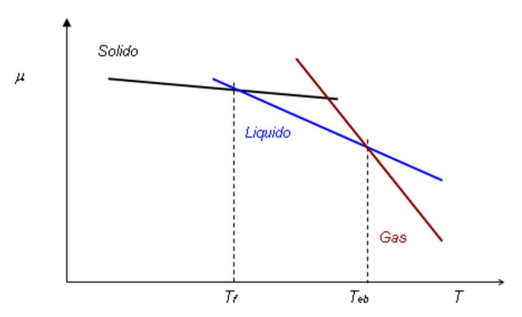
\includegraphics[width=0.5\linewidth]{Immagini/Potenziale chimico in funzione di T per un componente puro.png}
    \caption{potenziale chimico in funzione di $T$ per un componente puro.}
    \label{fig:Potenziale chimico in funzione di T per un componente puro}
\end{figure}

\subsection{Diagrammi di fase per un singolo componente}
A pressioni sufficientemente alte e/o temperature sufficientemente basse, la materia esiste allo stato solido. Ad elevate temperature e basse pressioni il gas è la fase stabile.
\begin{figure}[ht]
    \centering
    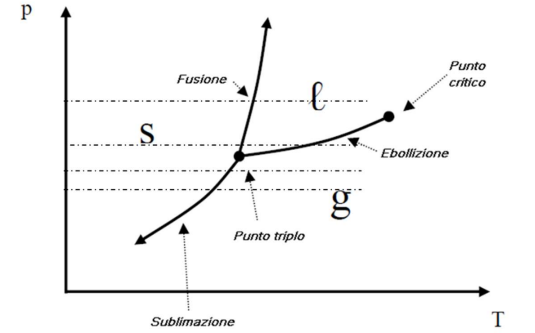
\includegraphics[width=0.5\linewidth]{Immagini/Diagramma di fase per un singolo componente.png}
    \caption{Diagramma di fase per un singolo componente}
    \label{fig:diagramma di fase per un singolo componente.}
\end{figure}

I diagrammi di fase forniscono un modo diretto di rappresentare il comportamento delle fasi. Sperimentalmente i diagrammi di fase sono costruiti misurando le temperature di fusione ed ebollizione (o di sublimazione) a diversi valori di pressione. Le linee sul diagramma indicano il set di condizioni in cui due fasi sono in equilibrio.

La coesistenza delle due fasi è descritta da $T(p)$ o $p(T)$, quindi una linea sul diagramma $pV$. Al punto triplo le tre fasi coesistono, il che significa che i potenziali chimici delle tre fasi sono uguali
\begin{equation}
    \mu_{\left(s\right)}(T,p)=\mu_{\left(l\right)}(T,p)=\mu_{\left(g\right)}(T,p),
\end{equation}
ottenendo due equazioni e due variabili.

Al punto critico la linea di demarcazione gas-liquido si interrompe. Oltre questo punto fase liquida e gas diventano indistinguibili e coesistono in un'unica fase (supercritica). Il punto critico rappresenta la massima temperatura a cui un gas può essere liquefatto semplicemente incrementando la pressione. 

Consideriamo un singolo componente distribuito su due fasi, fase $\alpha$ e fase $\beta$, all'equilibrio,in date condizioni di temperatura e pressione. Consideriamo una piccola quantità di moli $dn$ trasferita dalla fase $\alpha$ alla fase $\beta$ . La variazione di energia libera $dG$ è
\begin{equation}
    dG_\alpha=-\mu_\alpha dn,\quad dG_\beta=\mu_\beta dn,
\end{equation}
e la variazione di energia libera totale è
\begin{equation}
    dG=\left(\mu_\beta-\mu_\alpha\right)dn.
\end{equation}
Quando il sistema è all'equilibrio, $dG=0$, da cui $\mu_\alpha=\mu_\beta$. Questo fatto può essere generalizzato per qualunque numero di fasi.
\begin{teo}[fasi di un sistema all'equilibrio]
    A pressione e temperatura costanti, un sistema è all'equilibrio quando il potenziale chimico di un componente è lo stesso in ciascuna fase. 
\end{teo}

\subsection{Effetto delle condizioni esterne su \texorpdfstring{$\bm{\mu}$}{potenziale chimico}}
Per interpretare la pendenza delle curve di demarcazione tra le fasi nel diagramma di stato $(p,T)$, dobbiamo trovare una relazione per $dp/dT$ all'equilibrio tra le fasi, ovvero trovare l'effetto della dipendenza del potenziale chimico da pressione e temperatura. 

Si è visto che per due generiche fase $\alpha$ e $\beta$, sulla linea di
coesistenza delle fasi, $\mu_\alpha=\mu_\beta$. Considerando ora una variazione di temperatura $dT$ e di pressione $dp$, si ha
\begin{equation}
    \begin{cases}
        \mu_\alpha\left(T,p\right)\to\mu_\alpha\left(T,p\right)+d\mu_\alpha\left(T,p\right) \\ \mu_\beta\left(T,p\right)\to\mu_\beta\left(T,p\right)+d\mu_\beta\left(T,p\right)
    \end{cases}.
\end{equation}
Rimanendo sulla linea di coesistenza si ha $d\mu_\alpha=d\mu_\beta$, ma poiché $d\mu=d\bar{G}-\bar{S}dT+V\bar{V}dp$, su di essa si ha
\begin{equation}
    -\bar{S}_\alpha dT+\bar{V}_\alpha dp=-\bar{S}_\beta dT+\bar{V}_\beta dp,
\end{equation}
da cui
\begin{equation}
    \left(\frac{dp}{dT}\right)_{coes.}=\frac{\bar{S}_\beta-\bar{S}_\alpha}{\bar{V}_\beta-\bar{V}_\alpha}=\left(\frac{\Delta \bar{S}}{\Delta \bar{V}}\right)_{\alpha\to\beta}.
\end{equation}
Inoltre, ricordando che $\mu=\bar{G}=\bar{H}-T\bar{S}$, si può scrivere $\bar{H}_\alpha-T\bar{S}_\alpha=\bar{H}_\beta-T\bar{S}_\beta$, ovvero $\Delta \bar{H}_{\alpha\to\beta}=\left(T\Delta \bar{S}\right)_{\alpha\to\beta}$. In questo modo si ottengono le due forme dell'equazione di Clapeyron
\begin{equation}
    \begin{cases}
        \left(\dfrac{dp}{dT}\right)_{coes.}=\left(\dfrac{\Delta \bar{S}}{\Delta \bar{V}}\right)_{\alpha\to\beta} \\
        \left(\dfrac{dp}{dT}\right)_{coes.}=\left(\dfrac{\Delta \bar{H}}{T\Delta \bar{V}}\right)_{\alpha\to\beta}.
    \end{cases}
\end{equation}
Con queste equazioni si può interpretare il diagramma di fase. 

Considerando la transizione liquido-gas, avremo che la variazione di entropia è positiva, inoltre la variazione del volume molare nel passaggio liquido gas è positiva e grande, per cui
\begin{equation}
    \Delta \bar{S}>0,\,\Delta \bar{V}\gg0\Rightarrow\left(\frac{dp}{dT}\right)_{coes.}=\left(\frac{\Delta \bar{S}}{\Delta \bar{V}}\right)_{l\to g}>0,\quad(piccolo).
\end{equation}
Nel caso della transizione solido-gas, la variazione di entropia è maggiore rispetto al caso precedente, per cui
\begin{equation}
    \Delta \bar{S}\gg0,\,\Delta \bar{V}\gg0\Rightarrow\left(\frac{dp}{dT}\right)_{coes.}=\left(\frac{\Delta \bar{S}}{\Delta \bar{V}}\right)_{s\to g}>0,\quad(pi\grave{u}\,grande).
\end{equation}
Infine, nel caso del passaggio solido-liquido, si avrà per la maggior parte delle sostanze $\bar{V}_l   \geq\bar{V}_s$ e $\bar{S}_l>\bar{S}_s$, per cui
\begin{equation}
    \left(\frac{dp}{dT}\right)_{coes.}=\left(\frac{\Delta \bar{S}}{\Delta \bar{V}}\right)_{s\to l}>0,\quad(elevato).
\end{equation}
\begin{obs}
    Nel caso dell'acqua invece si ha $\bar{V}_l<\bar{V}_s$ e $\bar{S}_l>\bar{S}_s$, per cui
    \begin{equation}
        \left(\frac{dp}{dT}\right)_{coes.}=\left(\frac{\Delta \bar{S}}{\Delta \bar{V}}\right)_{s\to l}<0.
    \end{equation}
\end{obs}

\subsection{Soluzioni ideali e proprietà colligative}
La composizione di una soluzione può essere descritta in modi diversi. I più comunemente usati sono la molarità e la frazione molare.
\begin{defn}[molarità]
    \begin{equation}
        \textit{Molarità}=\frac{\textit{moli\,di\,soluto}}{litri\,di\,soluzione}.
    \end{equation}
\end{defn}
\begin{defn}[frazione molare]
La frazione molare $\chi_A$ di un componente A di una soluzione è data da
    \begin{equation}
        \chi_A=\frac{n_A}{n_A+n_B},
    \end{equation}
    dove $n_A$ e $n_B$ sono le moli di A e B nella soluzione A+B.
\end{defn}
Un soluzione ideale è caratterizzata da componenti che danno origine ad interazioni intermolecolari di natura
simile. Ci si limita a questi casi.
\begin{defn}[pressione di vapore]
    La pressione di vapore (o tensione di vapore) corrisponde alla pressione della fase gas in equilibrio con la fase liquida.
\end{defn}
Verso la fine del XIX secolo Francois Raoult riportò che per un gran numero di casi, vale la seguente legge.
\begin{axiom}[legge di Raoult]
    La pressione di vapore $p_i$ esercitata da un componente di una soluzione è proporzionale alla sua concentrazione espressa in termini di frazione molare $\chi_i$ secondo
    \begin{equation}
        p_i=\chi_ip_i^*,
    \end{equation}
    dove $p_i^*$ è la pressione di vapore del componente $i$ puro.
\end{axiom}
\begin{figure}[h]
    \centering
    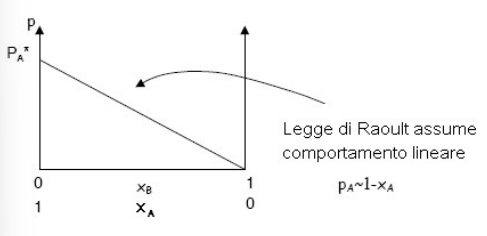
\includegraphics[width=0.5\linewidth]{Immagini/Illustrazione grafica della legge di Raoult.png}
    \caption{illustrazione grafica della legge di Raoult.}
    \label{fig:Raoult}
\end{figure}

 Considerando la soluzione A+B si ha
\begin{equation}
\begin{cases}
    p_A=p_A^*\chi_A \\
    p_B=p_B^*\chi_B \\
    p_{TOT}=p_A+p_B=p_A^*\chi_A+p_B^*\chi_B
\end{cases},\quad\chi_A=\left(1-\chi_B\right)
\end{equation}
Si considerino ora due contenitori alla stessa temperatura in situazione di equilibrio. Il contenitore 1 contiene il liquido puro A così che la pressione di vapore nel contenitore sarà $p_A^*$. Il secondo contenitore contiene una soluzione A+B con frazioni molari $\chi_A$ e $\chi_B$. Sulla base degli equilibri di fase prima visti, all'equilibrio il potenziale chimico di A dev'essere lo stesso in tutte le fasi.
\begin{figure}[h]
    \centering
    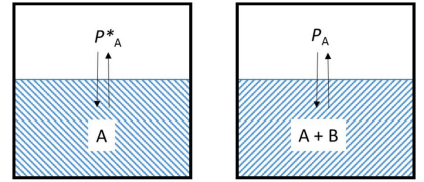
\includegraphics[width=0.5\linewidth]{Immagini/conten.png}
    \caption{contenitore: (i) 1; (ii) 2.}
    \label{fig:C}
\end{figure}

\noindent
Quindi
\begin{equation}\label{eq:sistema pot.chimico}
    \begin{cases}
        \mu_A\left(gas,p_A^*\right)=\mu_A\left(A,liquido,puro\right) \\
        \mu_A\left(gas,p_A\right)=\mu_A\left(A,soluzione,\chi_A\right).
    \end{cases}
\end{equation}
Dalla sezione \ref{sec: potenziale chimico} si ha
\begin{equation}\label{eq:sistema pot.chimico II}
    \begin{cases}
        \mu_A\left(gas,p_A^*\right)=\mu_A^\circ+RT\ln{\dfrac{p_A^*}{p_A^\circ}} \\[2ex]
        \mu_A\left(gas,p_A\right)=\mu_A^\circ+RT\ln{\dfrac{p_A}{p_A^\circ}}.
    \end{cases}
\end{equation}
Sottraendo la seconda dalla prima dal sistema \eqref{eq:sistema pot.chimico II} si ha
\begin{equation}
    \mu_A\left(gas,p_A\right)-\mu_A\left(gas,p_A^*\right)=\mu_A^\circ+RT\ln{\left(\frac{p_A}{p_A^*}\right)}
\end{equation}
Dalle relazioni del sistema \eqref{eq:sistema pot.chimico} si ha
\begin{equation}
     \mu_A\left(soluzione,\chi_A\right)-\mu_A\left(A,liquido,puro\right)=\mu_A^\circ+RT\ln{\left(\frac{p_A}{p_A^*}\right)}.
\end{equation}
Definendo lo stato standard come il liquido puro con potenziale chimico $\mu_A^\circ$ e il potenziale chimico del componente A nella soluzione come $\mu_A$ si ottiene
\begin{equation}\label{eq:mu(mustd)}
    \mu_A=\mu_A^\circ+RT\ln{\left(\frac{p_A}{p_A^*}\right)}.
\end{equation}
Si noti che l'unica assunzione fatta nel derivare questa relazione è che la fase gas abbia un comportamento ideale. L'equazione \eqref{eq:mu(mustd)} è del tutto generale e non comporta nessun tipo di assunzione sulle proprità della soluzione. Nel caso delle soluzioni ideali vale la legge di Raoult e si ha
\begin{equation}\label{eq:mu(mustd)Raoult}
    \mu_A=\mu_A^\circ+RT\ln{\left(\chi_A\right)}.
\end{equation}
Considerando che poiché $\chi_A<1$ si ha
\begin{equation}
    \mu_A\left(l,T,p\right)\left(soluzione\right)\leq\mu_A^*\left(l,T,p\right)\left(solvente\,puro\right)
\end{equation}
Ovvero il potenziale chimico di una soluzione è sempre minore di quello del solvente puro. Da questo fatto traggono origine le proprietà colligative delle soluzioni: abbassamento della tensione di vapore, innalzamento ebullioscopico, abbassamento crioscopico e pressione osmotica. 

\subsubsection{Pressione osmotica}
Il fenomeno dell'osmosi corrisponde alla tendenza del solvente puro a spostarsi in una soluzione da cui lo separa una membrana semipermeabile. Questa tendenza spontanea è il diretto risultato del fatto che il potenziale chimico del componente puro è maggiore di quello del componente in soluzione. Considerando i due punti indicati con $\alpha$ e $\beta$ in figura avremo che la pressione in questi due punti è data da
\begin{equation}
    \begin{cases}
        P_\beta=P_{est}+\log{\rho} \\
        P_\alpha=P_{est}+\log{\rho}+hg\rho=P_\beta+hg\rho=P_\beta+\Pi.
    \end{cases}
\end{equation}
\begin{figure}[ht]
    \centering
    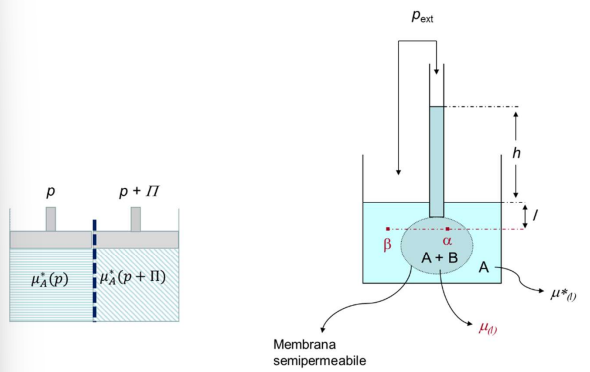
\includegraphics[width=0.7\linewidth]{Immagini/prs osm.png}
    \caption{esempi di applicazione della pressione osmotica.}
    \label{fig:osm}
\end{figure}

Il potenziale chimico di A nel solvente puro (punto $\beta$) e nella soluzione (punto $\alpha$) sarà dato da
\begin{equation}
    \begin{cases}
    \mu_A^\alpha=\mu_A\left(l,T,p+\Pi\right) \\
    \mu_A^\beta=\mu_A^*\left(l,T,p\right).
\end{cases}
\end{equation}
All'equilibrio deve essere $\mu_A^\alpha=\mu_A^\beta$ e usando l'equazione \eqref{eq:mu(mustd)Raoult} si può scrivere
\begin{equation}
    \mu_A^\alpha=\mu_A^*\left(l,T,p+\Pi\right)+RT\ln{\chi_A}=\mu_A^\beta.
\end{equation}
Considerando che il processo avvenga a temperatura costante, segue che
\begin{equation}
    dG=-SdT+Vdp=Vdp\Rightarrow d\mu_A^*=\bar{V}_A^*dp.
\end{equation}
Quindi
\begin{equation}
    \int_{p}^{p+\Pi}\bar{V}_A^*dp=\bar{V}_A^*\Pi=\mu_A^*\left(l,T,p+\Pi\right)-\mu_A^*\left(l,T,p\right).
\end{equation}
Assumendo $\bar{V}_A^*$ (volume molare di A) costante al variare di $p$ si ha che
\begin{equation}
    RT\ln{\chi_A}+\bar{V}_A^*\Pi=0.
\end{equation}
Ricordando che $\ln{\left(1-\chi_B\right)}\approx-\chi_B$, che $\chi_B=n_B/\left(n_A+n_B\right)\approx n_B/n_A$ e considerando che $\bar{V}_A^*\approx\bar{V}_A$ e che $n_A\bar{V}_A=V_A$ (volume del solvente), si ottiene
\begin{equation}
    RT\left(\frac{-n_B}{n_A}\right)+\frac{V_A}{n_A}\Pi=0,
\end{equation}
da cui si ottiene l'equazione di Van't Hoff
\begin{equation}
    \Pi V=n_BRT.
\end{equation}